\chapter{Konzeption} % Das würde eigentlich 'Konzeption' heißen aber Tichy wirkt stark in mir

hier kurz beschreiben, was so grob abgeht, also was wir so machen wollen und was für netze wir vergleichen wollen,
um das beste zu finden

\section{Datensatz für Fahrradwege}


\section{Pre-Processing} \label{sec:pre-processing}

Dieser Abschnitt befasst sich mit dem Pre-Processing, welches auf den in \autoref{sec:bike-data} 
beschriebenen Datensatz angewandt wird. Insbesondere ist die Klassenimbalance, Eingabegröße, 
Training-Validation-Test-Split und die Daten-Augmentation zu diskutieren. \\
Für die Verwendung im Modell werden die Pixelwerte aller Bilder von $[0; 255] \subset \mathbb{N}$
auf $[0;1] \subset \mathbb{R}$ abgebildet, indem alle Kanäle - bei RBG drei, bei den Graustufen-Masken einer - durch 255 geteilt werden.
Dies vermindert die betragsmäßige Größe der Eingaben und aufgrund der Masken auch Ausgaben. 

\subsection{Eingabegröße und Klassenimbalanceausgleich}

Durch die Art des Problems besteht bei der Erkennung der Fahrradwege ohnehin schon eine starke 
Klassenimbalance zwischen den Radweg-Pixel und den Hintergrundpixel. Diese Diskrepanz ist noch ein mal drastischer 
als bei den Straßendatensätzen, wo es schon ein Problem darstellt. So ist auf einem Bild mit Radweg 
tendenziell sehr wenig Radweg, aber sehr viel sonstige Strukturen, wie Vegetation, Gebäude und Straßen. 
Durch die automatische Generierung des Radweg-Datensatzes sind zudem viele Bilder von kleinen Orten,
Industriegebieten, Feldern und Wäldern vorhanden, die keinerlei eingezeichnete Radwege besitzen. 
Selbst in Bildern der Innenstadt haben oft nur größere Straßen dedizierte Radwege, während der 
Großteil des Bildes mit Wohngebiet gefüllt ist. 
Somit ist nur ein verschwindender Anteil aller Pixel des Datensatzes als Radweg markiert. 

Um den Anteil an Radwegpixel zu erhöhen, sollen nur Bilder zum Training verwendet werden,
die überhaupt Radwege enthalten. Da es technisch zu ressourcenaufwendig wäre ein ganzes 
$10.000 \times 10.000$-Pixel-Bild einzugeben, sollen die Bilder in kleinere Stücke zerteilt werden. 
Dies ist auch bei den Modellen zur Straßenerkennung aus \autoref{sec:state-of-the-art-roads} die Praxis. 
Vorgeschlagene Ausschnittsgrößen könnten hierbei $256\times 256$, $512\times 512$ und $1024 \times 1024$ sein. 
Wird ein größerer Ausschnitt gewählt, steigt potentiell die Klassenimbalance, da häufig viele überflüssige 
Hintergrundpixel eingeschlossen werden, allerdings kein weiterer Radweg im Bild liegt. 
Wird eine kleine Größe gewählt, könnte es sein, dass nur noch Radwege im Bild vorhanden sind, 
wodurch die Gefahr besteht, dass jede beliebige Straße einen Radweg seitlich angezeichnet bekommt. 
Es wären hauptsächlich große Straßen abgebildet -- kleine Straßen würden kaum gelernt werden. 
Außerdem würde es häufiger dazu kommen, dass Radwege nur sehr klein in den Ecken eines kleinen Bildausschnittes 
vorkämen und die lange zusammenhängende Struktur, die zu einem Radweg gehört, schwierige zu erlernen wäre. 
Aus diesen Gründen wird als Kompromiss die $512 \times 512$-Größe gewählt. Somit entspricht eine Bildkante 
$512 \cdot 0,2m = 102,4m$. Die Zweierpotenz bzw. eher das Vielfache von 32 wird daher gewählt, 
sodass das Bild nicht zu klein in der U-Net-Struktur wird, bzw. damit eine saubere Teilung der 
Max-Pool-Schichten möglich ist, die die Bildkantenlänge stets halbieren. 

\begin{wrapfigure}{r}{0.40\textwidth}
	\centering
	\vspace{-30pt} % Manchmal möchte man den oberen Abstand selbst anpassen
	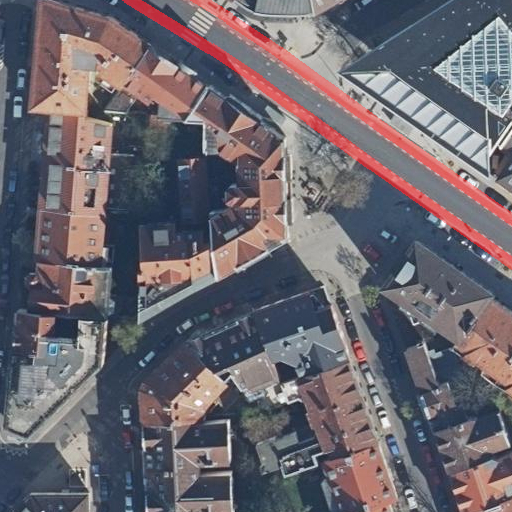
\includegraphics[width=0.35\textwidth]{Bilder/cut-example.jpg}
	\vspace{-10pt}
	% Das folgende ist ein Trick, um "Abbilgung x.y" in eine
	% eigene Zeile zu packen. Der Text zwischen [ und ] steht
	% im Abbildungsverzeichnis. Der Text darunter wird
	% tatsächlich angezeigt.
	\caption[Beispiel $512\times 512$-Ausschnitt aus Bike-Datensatz.]{\unskip}
	Beispiel $512\times 512$-Ausschnitt aus Bike-Datensatz mit roter Maske.
	\label{fig:cut-example}
\end{wrapfigure}

Jedes $10.000\times 10.000$-Pixel-Bild und die dazugehörige Maske wird in 
$\left\lceil{\frac{10.000}{512}}\right\rceil^2 = 400$ Teile geschnitten. 
Die 39 Ausschnitte, die nur partiell im Bild liegen, werden im überstehenden Bereich mit Schwarz ($RGB=(0,0,0)$) gefüllt.
Damit ergeben sich bei 143 Bildern $143 \cdot 400 = 57.200$ $512 \times 512$-Bildausschnitte. \\
Weiter werden alle Ausschnitte entfernt, die keine oder fast keine als Radweg annotierten Pixel beinhalten. 
Die Quote wird auf 1\% festgelegt. Sollte also ein Bildausschnitt weniger als 1\% Fahrradweg-Pixel beinhalten, 
wird es entfernt. Durch diese Maßnahme sinkt die Anzahl an Bildausschnitten von $57.200$ auf $10.181$ Bildausschnitte - 
dieser Anteil entspricht ca. 17,7\%. 
 
\autoref{fig:cut-example} zeigt beispielhaft ein auf $512\times 512$ Pixel zugeschnittenes Bild aus dem Bike-Datensatz 
mit der dazugehörigen Maske, die mit 50\% Transparenz in rot überlagert ist. Es ist zu erkennen, 
dass die Klassenimbalance noch recht stark ist, allerdings deutlich geringer, als in den ursprünglichen Bildern,
und dass auch trotzdem genügend Straßen ohne Radwege vorhanden sind und die Struktur und der Verlauf des Radweges 
bei der gewählten Ausschnittgröße weiterhin gut zu erkennen ist. 

\subsection{Training-Validation-Test-Split}

Zunächst werden die zerschnittenen Bilder aller Städte gemischt. Dann werden diese Ausschnitte disjunkt in 
Training-, Validation- und Test-Daten aufgeteilt. 
Damit sollten die unterschiedlichen Städte gleichermaßen in allen Teil-Datensätzen auftauchen, 
sodass der Test- und Validationdatensatz gut die Generalisierungsfähigkeit des Netzes überprüft. 
Durch die bereits höhere Zahl an Bildausschnitten (10.181 Stück) ist es eher unwahrscheinlich, 
dass eine ungleiche Verteilung der Städte vorkommt. Außerdem ist das Mischen wichtig, 
damit die Randausschnitte, die große schwarze Flächen beinhalten, anteilig gleich in 
jedem Teildatensatz repräsentiert sind, damit dies das Ergebnis nicht verfälscht, sollten diese 
zum Beispiel nur in dem Validation- oder Testdatensatz vorkommen. 

\autoref{tab:bike-split} zeigt den im Folgenden verwendeten Trainings-Validation-Test-Split. 
Hierbei sind zwei Dinge zu bemerken, die nicht aus der Tabelle hervorgehen: 
Zunächst wurde der Testdatensatz abgespaltet. Hierzu wurden 15\% vom Hannover-Teil und 
20\% von den jeweiligen restlichen Städten abgespaltet und vereinigt. Da der Hannover-Teil so groß ist, wie die restlichen 
Städte zusammen, läuft dies auf einen eher unkonventionellen Split von 17,5\% heraus. Diese Verteilung wurde so getroffen, 
um den Hannover-Teil etwas weniger zu gewichten, um im Test die Generalisierungsfähigkeit besser zu testen 
und den Einfluss der kleineren Städte zu erhöhen. Der Validation-Datensatz wurde danach aus 8\%, 
bzw. der Trainingsdatensatz aus 92\% vom Rest gebildet. \\
Der Trainingsdatensatz ist mit ca. 75\% der gesamten Daten eher groß gewählt. Diese Entscheidung wurde getroffen,
um möglichst viele und unterschiedliche Bilder zu verwenden, da der Datensatz mit automatischer Synthese 
generiert wurde und daher qualitativ eher unvorteilhaft ist, wodurch eine höhere Anzahl an Trainingsdaten nötig wird.

\begin{table}
	\centering
	\begin{tabular}{l|l|l|l|l}
		& Training & Val. & Test & Summe \\
		\midrule
		Absolut & 7738 & 672 & 1771 & 10181 \\
		Anteil & 75,9 & 6,6 & 17,5 & 100 \\ 
	\end{tabular}
	\caption{Training-Validation-Test-Split des Bike-Datensatzes in gefilterten $512 \times 512$-Ausschnitten.}
	\label{tab:bike-split}
\end{table}

Der Validationdatensatz wird genutzt, um nach jeder Trainingsepoche den Verlust dieses Datensatzes zu bestimmen. 
Verbessert sich der Validation-Verlust nach fünf Epochen nicht, wird die Lernrate um Faktor 10 verringert. 
Verbessert sich der Validation-Verlust nach sieben Epochen nicht, wird der beste Stand, mit der Epoche mit geringstem 
Validation-Verlust, wiederhergestellt und das Training vorzeitig beendet.  


\subsection{Augmentation}

Die Bild-Augmentation wird nicht vor dem Training angewandt, um den Datensatz künstlich zu vergrößern, 
sondern während dem Training pseudo-zufällig mit festem Seed, um die Ergebnisse reproduzieren zu können.
Somit wird jedes Bild während des Trainings, bevor es in das Netz eingegeben wird zufällig augmentiert 
und dann eingegeben. Somit erhält ein und dasselbe Bild über die verschiedenen Epochen jedes Mal unterschiedliche 
Anpassungen auf Basis des Zufallsgenerators. Dies erhöht deutlich die Generalisierungsfähigkeit bzw. 
verringert die Gefahr von Overfitting drastisch. Das Netz sieht tendenziell viel mehr Varianten der Bilder. 
Der einzige Nachteil ist, dass das Training tendenziell länger dauert, da jedes Bild vor Eingabe bearbeitet wird. 
Dieser Nachteil ist vor allem evident, wenn mehrere Netze auf demselben Datensatz trainiert werden, da jedes mal 
dieselben Augmentationen (da gleicher Seed) erneut vorgenommen werden müssen. Dieses Problem könnte allerdings
durch eine Vorausberechnung der aufeinanderfolgenden Augmentationen behoben werden. 
Die Verlängerung pro Epoche lag allerdings lediglich bei zwei Minuten beim Bike-Datensatz und fünf Minuten beim Pre-Training auf der 
Straßenerkennung, daher wurde auf den zusätzlichen Aufwand einer solchen Implementation verzichtet 
(vgl. eine Epoche benötigt im Schnitt 10-17 min bzw. 40-50 min). 

Jede der folgenden Augmentationen wird in ihrem Wertebereich pseudo-zufällig angewandt. Sollte es die Veränderung 
erfordern, werden fehlende Bildteile mit Schwarz gefüllt. Schwarz wurde ausgewählt, da es ohnehin Bilder mit 
schwarzen Rändern im Datensatz gibt, weswegen das hierbei mit nichts Neuem konfrontiert ist. 
\begin{enumerate}
	\item Rotation im Intervall von $[-90^\circ ; 90^\circ ]$. Eine Gradzahl wird für jedes Bild zufällig ausgewählt und angewandt. 
	Die dabei entstehenden leeren Bildbereiche werden mit Schwarz ($RGB = (0,0,0)$) gefüllt. 
	Diese Augmentation ist realistisch und nützlich, da Straßen in beliebiger Ausrichtung vorkommen und 
	eine natürliche Orientierung bei Bildern aus der Vogelperspektive nicht besteht.
	\item Horizontale Spiegelung. Es wird zufällig entschieden, ob ein Bild an der vertikalen Spiegelachse gespiegelt wird. 
	Diese Augmentation ist ebenfalls realistisch und hat gegenüber der Rotation den Vorteil keine schwarzen Flächen 
	einzuführen aber den Nachteil nicht so viele neue Bilder erzeugen zu können. 
	\item Vertikale Spiegelung. Wie horizontale Spiegelung, allerdings wird an der horizontalen Achse gespiegelt. 
	Beide Spiegelungen können simultan auftreten, es gibt also vier Spiegelungs-Permutationen, 
	die mit gleicher Wahrscheinlichkeit auftreten.
	\item Horizontale Verschiebung im Intervall von $[-0,1 \cdot w; 0,1 \cdot w]$ Pixel entlang der horizontalen Achse,
	wobei $w$ die Breite des Bildes ist. Es wird eine zufällige Länge aus dem Intervall ausgewählt und verschoben; die 
	entstehenden Ränder werden mit Schwarz gefüllt. Auch diese Augmentation ist realistisch und erhöht lediglich 
	die Möglichkeit der Veränderung der Bilder. 
	\item Vertikale Verschiebung im Intervall von $[-0,1 \cdot h; 0,1 \cdot h]$ Pixel entlang der vertikalen Achse,
	wobei $h$ die Höhe des Bildes ist. Rest wie bei der horizontalen Verschiebung.    
\end{enumerate} 

\autoref{fig:augmentation} zeigt eine beispielhafte Augmentierung des Bildes und der dazugehörigen Maske aus \autoref{fig:cut-example},
wobei eine horizontale Spiegelung\footnote{Die Spiegelachse ist hierbei \textit{vertikal}.},
eine Rotation um 13° und eine Verschiebung um 8\%, also $\lceil 0,08 \cdot 512 \rceil = 41$ Pixel, 
nach links dargestellt ist. Es ist keine vertikale Spieglung oder vertikale Verschiebung vorhanden.
Die Randbereiche, wofür aufgrund der Verschiebung und Rotation keine Daten vorhanden sind, sind mit Schwarz gefüllt. 

Die angewandten Augmentationen sind eher konservativ gewählt. An den Bildern wird kaum etwas verändert, 
außer die Pixel leicht umzusetzen. Dadurch würde ein augmentiertes Bild im Original-Datensatz nicht auffallen. 
Auf weitergehende Veränderungen wie Gamma-Korrektur, Helligkeitsanpassung, Zoom und Scherung wird hingegen verzichtet. 
Diese Veränderungen werden nicht vorgenommen, um mit dem Testdatensatz besser Abschätzen zu können, 
wie gut die Erkennung der Radwege allgemein - unter optimalen Bedingungen - funktioniert, ohne zunächst auf 
maximale Generalsierungsfähigkeit zu untersuchen. Diese Abschätzung wird dann mithilfe des Testdatensatzes von 
Karlsruhe, welcher im Erscheinungsbild stark vom Bike-Testdatensatz abweicht, vorgenommen, 
indem die Ergebnisse für den Bike-Testdatensatz und den Karlsruhe-Datensatz verglichen werden. \\
An dieser Stelle sei jedoch gesagt, dass insbesondere die Zoom-Augmentation sehr nützlich sein könnte, 
sollte das Modell für Orhtofotos mit unterschiedlicher \ac{GSD} generalisiert werden. 

Am Ende jeder Epoche wird der Trainingsdatensatz gemischt, sodass in der nächsten Epoche neue zufällige 
Batches entstehen. 

\begin{figure}
	\centering
	\begin{minipage}{.45\textwidth}
		\centering
		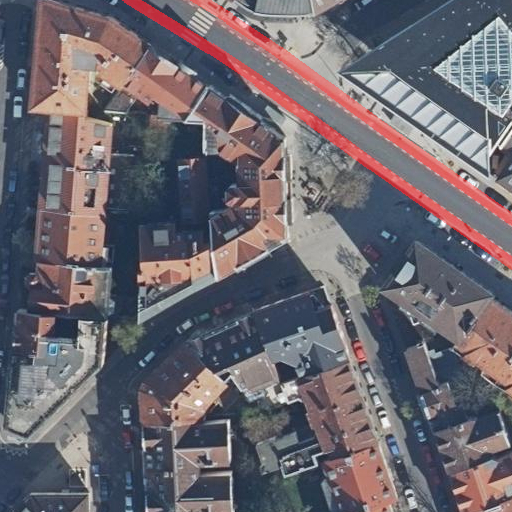
\includegraphics[width=.7\linewidth]{Bilder/cut-example.jpg} 
	\end{minipage}
	\begin{minipage}{.45\textwidth}
		\centering
		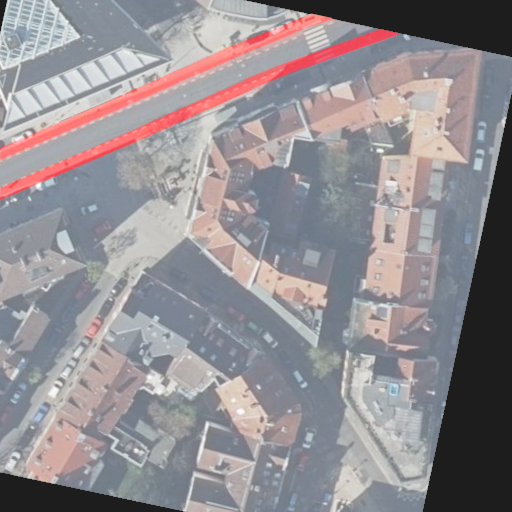
\includegraphics[width=.7\linewidth]{Bilder/augmentation-example.png} 
	\end{minipage}

	\caption{Beispielhafte Datenaugmentation mit Originalbild und Maske in Rot links 
	und augmentiertes (horizontale Spiegelung, Rotation, Verschiebung nach links) Bild 
	mit Maske in Rot rechts.  }
	\label{fig:augmentation}
\end{figure} 

% augmentation = {
% 	"rotation_range": 90,
% 	"width_shift_range": 0.1,
% 	"height_shift_range": 0.1,
% 	"fill_mode": "constant",
% 	"cval": 0,
% 	"horizontal_flip": "True",
% 	"vertical_flip": "True",
% 	"validation_split": 0.08

\section{Architektur} \label{sec:architecture}

Im Folgenden werden die untersuchten Architekturen genauer beschrieben und ebenfalls begründet, 
warum die jeweiligen architektonischen Entscheidungen getroffen wurden. \\
In \autoref{sec:state-of-the-art-roads} wurde ausführlich der Stand der Technik und Wissenschaft 
im Bereich der Straßenerkennung und -extraktion mittels Computer-Vision-Modellen beschrieben. 
Aufgrund der Ähnlichkeit der Problemdomäne lässt sich vermuten, dass ähnliche Verfahren wie 
zum Erkennen von Straßen auch für das Erkennen von Fahrradwegen nützlich sein könnten. 
Die Problemdomänen sind ähnlich, da Fahrradwege auch Straßen sind und eben jene Eigenschaften, 
wie große Klassenimbalance zwischen Fahrradweg und Hintergrund, Beschattung durch andere Objekte,
Verdeckung durch z.B. Bäume und ähnliche Annotationsfehler   
teilen. Schwierigkeit hier wird sein, Fahrradwege von Straßen zu unterscheiden. \\
Die Radwege sollen, wie Straßen auch, mittels Image-Semantic-Segmentation von einem Computer-Vision-Modell 
markiert werden. Andere Klassifizierungsarten, wie die in \autoref{sec:aufgabenkategorien} beschriebene 
Objektdetektion würde zu grobe Bounding-Boxes um schräg verlaufende Radwege legen, sodass im Prinzip 
eine Straße markiert werden würde, die zwar ein Radweg hat, aber nicht klar wäre, wo dieser verläuft, 
bzw. ob ein Radweg in beide Richtungen existiert. Aus demselben Grund ergibt eine reine Klassifikation, 
ob ein Bild ein Radweg enthält oder nicht ebenfalls keinen Sinn. 
Auf der anderen Seite würde Instanz-Segmentierung keine weiteren relevanten Informationen hinzufügen, 
wonach semantische Segmentierung völlig ausreicht, um das Problem zu lösen. \\
Wie bereits in \autoref{sec:state-of-the-art-roads} dargelegt sind alle relevanten Modelle zur 
Straßenerkennung basierend auf der U-Net-Archtiektur (vgl. \ref{sec:architekturkomponenten:unet}).
Folglich sollen die hier betrachteten Modelle ebenfalls als angepasste U-Nets entworfen werden. 
Insbesondere ermöglicht dies auch die Modelle zur Fahrradwegerkennung auf den verschiedenen 
in \autoref{sec:road-detection:roads-data} vorgestellten Datensätzen zur Straßenerkennung vorzutrainieren, 
was zu allgemein besseren Ergebnissen führen kann (s. \autoref{sec:transfer-learning}). 
Außerdem können so die erzielten Ergebnisse vom Pre-Training mit den öffentlichen Benchmarks verglichen werden,
um deren Ergebnisse zu validieren und früh Fehler in den eigenen Entscheidungen und Implementationen zu entdecken.

Zunächst soll so ein nur leicht modifiziertes U-Net, welches im Folgenden \textit{Bike-U-Net} 
genannt wird, entworfen werden, welches als Baseline- und Vergleichs-Netz dienen soll.
Dann soll eine zweite Klasse an U-Nets beschrieben werden, die verschiedene vortrainierte \acp{CNN} (s. \autoref{sec:pretrained-backbones}) 
als Backbones für ein U-Net verwendet, da \autoref{sec:state-of-the-art-roads} gezeigt hat, 
dass im Falle der Straßendetektion die Performanz eines Netzes stark verbessert werden konnte, 
indem auf Techniken und Methoden von Modellen aus anderen Teilgebieten der Computer-Vision 
zurückgegriffen wurde. Die einfachste Ausprägung hiervon ist das Dense-U-Net-121, 
welches einfach ein DenseNet121 als Backbone verwendet und somit von dessen Pre-Training und Architektur
profitieren konnte und damit 2-5\% bessere Resultate in der Basline-Bewertung und bis zu 19\% 
bessere Ergebnisse in der optimierten Version erzielen konnte, als ein herkömmliches U-Net. 
Gegebenenfalls ist das auch für die Radwegerkennung möglich. Dazu sollen mehrere Backbones untersucht werden. 

\subsection{Bike-U-Net} \label{sec:architecture:bike-u-net}

\autoref{fig:bike-unet-2} zeigt die von uns verwendete Architektur für das \textit{\ac{BUNet}}, 
bzw. genauer das \textit{\ac{BUNet2}}. Hierfür wurde das in \autoref{fig:u-net-architecture} 
dargestellte originale U-Net auf den vorliegenden Anwendungsfall angepasst.
Diese Anpassungen sind in der nachfolgenden Liste erklärt.

\begin{itemize}
	\item Zunächst werden Input-Bilder der Größe $width \times height \times 3$ verwendet. 
	Wobei $width$ und $height$ variabel in der Architektur sind, mit der Einschränkung, 
	dass diese Vielfache von 32 sein sollten, damit die mittlere Schicht nicht zu klein wird. 
	In jedem Fall wird ein drei-kanal RGB-Bild verwendet. In der Abbildung ist exemplarisch $512 \times 512 \times 3$ gewählt. \\
	Der Output verwendet zunächst keine explizite One-Hot-Kodierung für Fahrradweg und Hintergrund, 
	sondern eine implizite, wie in \autoref{sec:state-of-the-art-roads} beschrieben, 
	um eine intuitivere Bewertung zu erhalten. 
	\item Im Gegensatz zum originalen U-Net, wird bei den Convolutional-Layern Padding eingesetzt,
	um die Dimensionen der Feature-Maps nicht nach und nach zu verkleinern und so einen exakt symmetrischen Aufbau zu gewährleisten.
	Ebenso wurde bei den Up-Convolutions Padding eingefügt, um auch hier eine Verkleinerung der Feature-Maps zu verhindern.
	Diese Anpassung wurde eingesetzt, um kein Zuschneiden bei den Skip-Connections zu benötigen, was die Lokalisierung verbessern soll,
	und so bei den in \autoref{sec:state-of-the-art-roads} beschriebenen Netzen gewöhnlich ist.
	\item Im originalen U-Net beginnt der erste Convolutional-Block mit 64 Filtern, 
	welche sich jeden weiteren Block mit zum Mittel-Block verdoppeln, der dann 1024 Filter besitzt.
	Daraufhin halbieren sich die Filter mit jedem weiteren Decoder-Block wieder. \\
	Im Bike-U-Net-2 beginnen die Filter bei 16 und verdoppeln sich bis 256, was zu ungefähr 2 Mio. 
	trainierbaren Parametern führt. Die Zahl an Parametern ist somit weitaus geringer als im 
	Original-U-Net mit ca. 24 Mio. Parameter \cite{Ronneberger.18052015}. 
	Hiermit soll getestet werden, ob auch ein recheneffzienteres und kleineres U-Net gute Ergebnisse liefert, 
	und somit auch weniger Regularisierung notwendig ist. \\
	Da aber die in \autoref{sec:state-of-the-art-roads} beschriebenen Netze ebenfalls 15-25 Mio. Parameter haben, 
	soll ein weiteres U-Net mit mehr Parametern getestet werden. Dieses \textit{\ac{BUNet15}} ist 
	abgebildet in \autoref{fig:bike-unet-15} und hat 15 Mio. Parameter. Dies wurde erzielt, 
	indem die Filter ab Block zwei dreimal mehr sind, als im Bike-U-Net-2. So haben wir hierbei 16 Filter in Block eins, 
	dann 96 Filter in Block zwei, die sich verdoppeln bis hin zu 768 Filtern im mittleren Block und danach wieder halbieren bis zum vorletzten Block. 
	Dabei hat der letzte Block wieder 16 Filter. 
	Der erste und letzte Block haben dabei jeweils 16 Filter, da damit der Rechen- und Speicheraufwand erheblich reduziert werden kann.
	Bis auf die Filteranzahl und die daraus resultierende Tiefe der Feature-Maps, sind Bike-U-Net-2 und Bike-U-Net-15 identisch.
	\item Auf jede Convolution-Schicht folgt eine Batch-Normalization-Schicht. 
	Dies hat mehrere Gründe: Zum einen übernimmt so das Netz selbst die Normalisierung und Standardisierung der Daten, 
	wodurch sich das beim Vorverarbeiten gespart werden kann und zum anderen kann von den in \autoref{sec:architekturkomponenten:batchnorm} 
	beschriebenen Vorteilen, wie schnellerem Training und leichter Regularisierung profitiert werden, 
	ohne, dass dafür zusätzlicher Aufwand betrieben werden muss und keine Nachteile entstehen.
	\item Zusätzlich zu den Batch-Normalization-Schichten wurden pro Block eine Dropout-Schicht 
	nach der jeweils ersten Convolution-Schicht eingezogen. Diese sollen als 
    Hyperparameter eingebaut werden, um einfach kontrollierbar Regularisierung anzuwenden, 
	sollten die Modelle Probleme mit Overfitting durch zu hohe Komplexität bekommen. 
	Aufgrund der eher wenigen Parameter wird dies aber gegebenenfalls nur beim Bike-U-Net-15, 
	oder überhaupt nicht nötig.
	\item Die Convolution-Schichten werden durch \ac{ELU} aktiviert, anstatt durch \ac{ReLU}, wie im Original-U-Net. 
	Hierdurch können die meisten der in \autoref{sec:activation} herausgearbeiteten Vorteile von \ac{ReLU},
	wie Robustheit gegen das Vanishing-Gradient-Problem, genutzt werden. Jedoch wurde bereits im ursprünglichen U-Net-Paper 
	(\cite{Ronneberger.18052015}) auf ein Problem hingewiesen, worunter oftmals \acp{CNN} leiden: Häufig kommt es vor, 
	dass Netzteile dauerhaft nicht oder nur kaum aktiviert werden und so kaum etwas beitragen. 
	Dieses Problem ist insbesondere für \ac{ReLU} relevant, da diese Aktivierungsfunktion unter dem Dyning-Neuron-Problem leidet.
	Deshalb wurde hier auf \ac{ELU} zurückgegriffen, da damit alle Netzteile zum Beitrag animiert werden sollen. 
	Der einzige Nachteil ist hierbei, dass die Berechnung von \ac{ELU} etwas aufwendiger ist. 
	Das Problem von unbeschränkt großen positiven Aktivierungen unter denen sowohl \ac{ELU} als auch \ac{ReLU} leiden,
	wird in diesem Netz durch die wiederholte Batch-Normalisierung abgefedert.
	\item Für das Ouptut-Layer, nach der $1\times 1$-Convolution, wird die Sigmoid-Funktion verwendet. 
	Im Falle einer One-Hot-Kodierung würde hier Softmax herangezogen werden. 
\end{itemize}

\begin{figure}
	\centering
	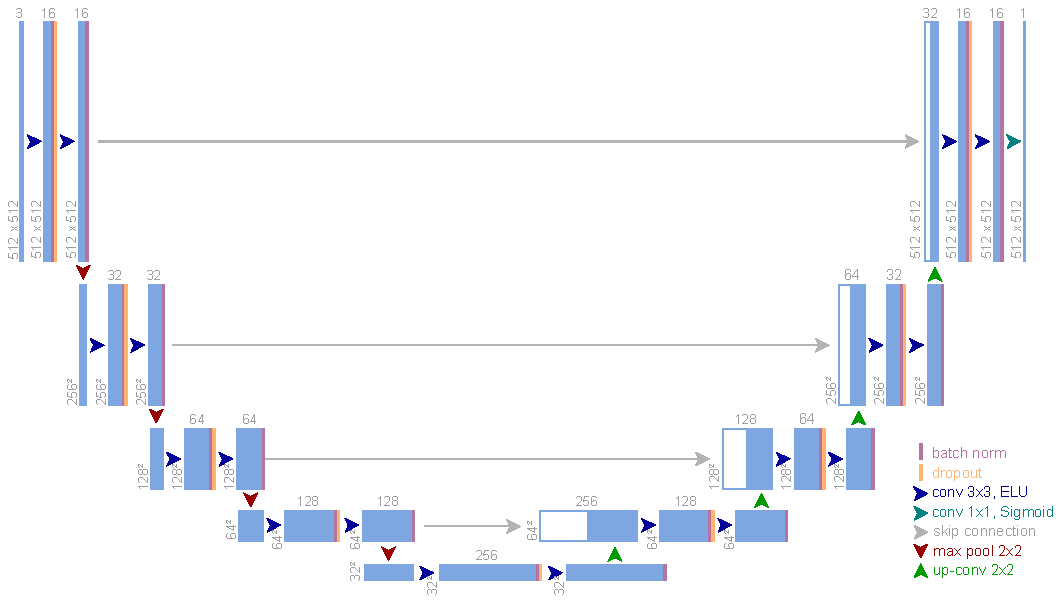
\includegraphics[width=1.\textwidth]{Bilder/own-unet-2mil.pdf} 
	\caption{Bike-U-Net-2 mit 1,946 Mio. Parametern.}
	\label{fig:bike-unet-2}
\end{figure} 

% HE INITIALIZATION

\subsection{Backbone-U-Nets}

Dieser Abschnitt beschreibt kurz die als U-Net mit vortrainiertem Backbone entworfenen Architekturen. \\
Prinzipiell dienen die Convolution-Schichten aller in \autoref{sec:pretrained-backbones} der Feature-Erkennung 
und -Extraktion. Lediglich die letzten Schichten, die bei den beschriebenen Klassifikationsmodellen allesamt 
Fully-Connected-Schichten waren, sind für die schlussendliche Zuordnung der Features zu den Objektklassen 
im ImageNet-Datensatz notwendig. Werden diese Schichten mit einem Decoder-Teil, der den Encoder - hier 
also das vortrainierte Klassifikationsnetz - spiegelt, entsteht ein Modell zur semantischen Segmentierung. 
Weiter müssen lediglich an geeigneter Stelle Skip-Connections zwischen Encoder und Decoder eingefügt werden,
um die U-Net-Form nachzubilden. Im Folgenden werden die auf diese Weise konstruierten Netze beschrieben. 

\subsubsection{VGG16-Bike-U-Net}

\textit{\ac{VBUNet}} nutzt das in \autoref{sec:pretrained-backbones:vgg16} beschriebene Netz VGG16 
mit auf ImageNet vortrainierten Gewichten als Backbone. \\
Hierzu werden die drei Fully-Connected-Layer 
(und Soft-Max-Aktivierung) am Ende entfernt und mit drei neuen \textit{conv3-512}-Schichten ersetzt. 
Diese bilden den mittleren (\enquote{untersten}) Block im U-Net. Darauf folgt eine direkte Spieglung 
von VGG16 als Decoder mit abschließender $1\times 1$-Convolution. Im Gegensatz zum Bike-U-Net (s. \autoref{sec:architecture:bike-u-net}) 
und ursprünglichen U-Net (s. \autoref{sec:architekturkomponenten:unet}) wurden allerdings keine 
\textit{up-conv3}-Layer mit trainierbaren Gewichten zum Upsampling genutzt, sondern 2D-Upsampling-Layer, 
ohne trainierbaren Parameter. Diese Entscheidung wurde getroffen, um VGG16 besser nachzuempfinden, 
da hier Maxpool-Schichten zum Downsampling verwendet werden, die ebenfalls keine trainierbaren Parameter enthalten.
Weiter sind nach jeder nicht-vortrainierten Convolution-Schicht, also nach jeder, die nicht zu VGG16 gehören, 
Batch-Normalization-Layer eingezogen, aus den in \autoref{sec:architecture:bike-u-net} und \autoref{sec:architekturkomponenten:batchnorm}
genannten Gründen wie schnellerem Training, leichter Glättung und fehlender sonstiger Standardisierung und Normalisierung.
Die für U-Net charakteristischen Skip-Connections werden vor jeder Maxpool-Schicht außer der ersten eingesetzt 
und mit dem korrespondierenden Decoder-Block verbunden. Dies resultiert in genau vier Skip-Connections, 
wie im Bike-U-Net und originellen U-Net. Abgeschlossen wird durch eine Sigmoid-Aktivierung, so wie im Bike-U-Net. \\
VGG16-Bike-U-Net enthält 23,7 Mio. Parameter. Grob die Hälfte davon (14,7 Mio.) sind von VGG16. 

VGG16 wird als Backbone ausgewählt und getestet, da es als eine Art Basis- bzw. Standardversion der nachfolgenden 
Backbone-Netze aufgefasst werden kann, da diese auf VGG16 aufbauen und dieses - zumindest 
für den ImageNet-Datensatz - verbessern und nachvollzogen werden soll, ob diese Anpassungen dienlich sind 
für den konkreten Anwendungsfall der Radwegerkennung. Zudem ist VGG16 sehr beliebt als vortrainiertes 
Netz, weswegen es viele Vergleichsmöglichkeiten gibt. 
Des Weiteren wird VGG16 als Backbone in Research zum Pre-Training mit U-Nets eingesetzt (s. \autoref{sec:transfer-learning:backbones}), 
auf dessen Ergebnisse diese Arbeit aufbaut. 
Demnach ist es wiederum für Vergleichszwecke sinnvoll VGG16 als Backbone für die Radwegerkennung zu verwenden.   

\subsubsection{ResNet34-Bike-U-Net}

\textit{\ac{RBUNet}} nutzt das in \autoref{sec:pretrained-backbones:resnet} beschriebene Netz ResNet34 
mit auf ImageNet vortrainierten Gewichten als Backbone. \\
Hierzu wird die eine Fully-Connected-Layer am Schluss des Netzes entfernt und um einen Decoder ersetzt. 
Anders als bei \ac{VBUNet} ist der mittlere Block der U-Net-Struktur von ResNet34 
und nicht zusätzlich neu ergänzt. Die Begründung hierfür liegt in der höheren Anzahl an Parametern 
von ResNet34, welche ohne die Fully-Connected-Schicht bereits bei 24,4 Mio. liegt, im Gegensatz zu VGG16. 
Da der mittlere Block die meisten Parameter beinhaltet wird keine weitere Vertiefung des Netzes vorgenommen,
um die Anzahl der Parameter nicht drastisch zu erhöhen. An Stelle dessen wird nach Ende der Convolution-Schichten von 
ResNet34 direkt mit dem Upsampling begonnen, welches wie bei \ac{VBUNet} mit Upsampling-Schichten 
bewerkstelligt wird. Auch wird im Widerspruch zu \ac{VBUNet} der Encoder - also ResNet34 - nicht gespiegelt, 
um eine Verdoppelung der Parameteranzahl zu vermeiden. Stattdessen wird ein einfacher, U-Net-ähnlicher Decoder
aus fünf Blöcken á Upsampling-Schicht und zwei Convolution-Schichten verwendet, wobei in jedem Block 
die Filter-Anzahl von 512 an bis schließlich 16 halbiert wird. Abgeschlossen wird wie bei \ac{VBUNet} und
\ac{BUNet} mit $1\times 1$-Convolution und Sigmoid-Aktivierung. Aus den gleichen Gründen wie bei \ac{VBUNet}
sind nach jeder Convoltuion-Schicht Batch-Normalization-Schichten eingezogen. 
Es erfolgt wiederum das Einsetzen von vier Skip-Connection nach U-Net-Vorbild ergänzend zu den 
Skip-Connections der Residuen-Blöcke an folgenden Stellen: 
nach der $7\times 7$-Convolution zu Beginn von ResNet34, 
am Ende der Blöcke mit 64 Filtern, am Ende der Blöcke mit 128 Filtern 
und am Ende der Blöcke mit 256 Filtern. Im Decoder werden diese jeweils 
zu Beginn der ersten vier Decoder-Blöcke konkateniert. \\ 
ResNet34-Bike-U-Net enthält 24,4 Mio. Parameter. Davon sind 21,2 Mio. von ResNet34 und lediglich 3,2 Mio. 
vom Decoder, welcher somit eher unterrepräsentiert ist im Netz.  

ResNet34 wird als Backbone ausgewählt und getestet, aufgrund der hohen Präsenz von 
Residual-Blöcken in den leistungsstärksten Modellen 
zur Straßenerkennung aus \autoref{sec:state-of-the-art-roads} und insbesondere \autoref{tab:optimized-benchmarks}.
Es wird sich ebenfalls eine bessere Performanz dieses Modells bei der Radwegerkennung erhofft. 

\subsubsection{DenseNet121-Bike-U-Net}

\textit{\ac{DBUNet}} nutzt das in \autoref{sec:pretrained-backbones:densenet121} beschriebene Netz DenseNet121 
mit auf ImageNet vortrainierten Gewichten als Backbone. \\
Hierzu wird die Classification-Layer bestehend aus einer $7\times 7$-Average-Pool-Schicht 
und einer Fully-Connected-Layer entfernt und durch einen Decoder ersetzt. 
Wie schon bei \ac{RBUNet} erstreckt sich das DenseNet bis in den mittleren U-Net-Block. Beim \ac{DBUNet} 
liegt der Grund dafür allerdings nicht in der hohen Parameterzahl, sondern in der hohen sonstigen Komplexität 
des Netzes. So benötigt DenseNet121 trotz deutlich geringerer Parameterzahl für die Inferenz und das Training länger 
als sowohl \ac{RBUNet}, als auch \ac{VBUNet}. Vermutlich ist hierfür die große Tiefe von 64 Schichten, wovon 
60 Convolution-Schichten sind, verantwortlich. Um die Inferenz- und Trainingszeit also nicht weiter zu belasten, 
ist der Decoder eher schmal gehalten. Für den Decoder wird die gleiche Architektur wie im \ac{RBUNet} verwendet.
Auch hier sind die Batch-Normalization-Schichten eingezogen. Der einzige Unterschied besteht darin, 
dass die erste Convolution-Schicht anders als bei \ac{RBUNet} nicht von 512 Kanälen auf 256 abbildet, 
sondern von 1536 auf 256. Dies liegt an der Konkatenierung der DenseNet-Architektur. Wieder wird das 
Netz abgeschlossen durch eine $1\times 1$-Convolution gefolgt von einer Sigmoid-Aktivierung. 
Auch hier werden wieder vier Skip-Connections eingebaut, um die U-Net-Architektur nachzuahmen. 
Diese Skip-Connections sind im Falle von \ac{DBUNet} im Encoderteil nach der ersten $7 \times 7$-Convolution 
und dann jeweils nach jeder weiteren $1\times 1$-Convolution der DenseNet-Transition-Zonen eingesetzt. 
Im Decoder-Teil sind diese wie bei \ac{RBUNet} zu Beginn jedes Decoder-Blocks bis auf den letzten eingebaut. \\
DenseNet121-Bike-U-Net enthält 12,1 Mio. Parameter, wovon 6,9 Mio. zum DenseNet121 und 5,1 Mio. neu hinzugefügt 
wurden. Trotz doppelter bzw. sogar vierfacher Tiefe besteht \ac{DBUNet} nur aus ungefähr halb so vielen 
Parametern wie \ac{RBUNet} und \ac{VBUNet}. 

DenseNet121 wird als Backbone ausgewählt, wegen der guten Ergebnisse von Dense-U-Net-121 aus \autoref{sec:state-of-the-art-roads}. 
Darüber hinaus werden zusammen mit VGG16 und ResNet34 Netze mit verhältnismäßig flacher, mitteltiefer und tiefer 
Architektur getestet, was eine Vielfalt an Architekturen abbildet.

\section{Evaluationsmaße}

Dieser Abschnitt beschäftigt sich mit der Auswahl geeigneter Bewertungsmaße für die Performanz des Netzwerkes. 
Insbesondere wird eine geeignete Verlustfunktion ermittelt. Die folgenden Diskussionen und 
Betrachtungen stützen sich auf \autoref{sec:evaluation-metrics} und die dort beschriebenen Maßzahlen.
Weiter ist zu beachten, dass sich sämtliche Maßzahlen auf eine implizite Bestimmung der Hintergrundpixel
durch ein Output-Neuron pro Pixel bezieht und nicht auf eine One-Hot-Kodierung. 

Als eine direkte und intuitiv sehr anschauliche Metrik zum Bewerten der Modellperformanz bei Segmentierungsproblemen
kann \ac{IoU} herangezogen werden. Die \ac{IoU} ist dabei auch ein recht verbreitetes Maß in der semantischen Segmentierung, 
weswegen es viele Vergleichswerte gibt, um die Modellperformanz bewerten zu können. \\ 
Problematisch an der \ac{IoU} dagegen ist, dass alle möglichen Klassifikationen ($tp$, $fp$, $fn$, $tn$)
gleich stark gewichtet werden, wobei die wahr-positiven $tp$ zunächst Priorität haben sollten, 
während die Fehler der falsch-positiven $fp$ und falsch-negativen $fn$ im Gleichgewicht bleiben sollten, 
sodass es nicht zu einer trivialen Klassifikation als rein positiv oder rein negativ kommt. \\
Ein weiteres Problem ist, dass die \ac{IoU} sehr streng und intolerant gegenüber leicher Verschiebung der Erkennung 
bewertet. Wenn ein Fahrradweg, der nur wenige Pixel breit ist, um die Hälfte der Breite verschoben segmentiert würde
aber ansonsten komplett dem Radweg entspricht, würde die \ac{IoU} bereits von 1 auf 0,5 sinken, obwohl \textit{qualitativ} 
der Weg exakt erkannt wurde. Diese Intoleranz gegenüber leichter lokaler Verschiebung ist insbesondere in dem 
in dieser Arbeit vorgestellten Bike-Datensatz aus \autoref{sec:bike-data} problematisch, 
da dieser über \ac{OSM} annotiert ist und für viele Straßen die Lage des zugehörigen Radwegs heuristisch über 
die Spuranzahl ermittelt wird. \\
Aufgrund der genannten Einschränkungen ist die \ac{IoU} ungeeignet als Verlustfunktion, kann jeoch als eine Dimension 
in der Bewertung miteinflißen. 

Das Quality-Maß adressiert das Verschiebungs-Problem der \ac{IoU} mit einem Buffer zur relaxierteren Ermittlung der 
$tp$, $fp$ und $fn$. Hierbei ist allerdings die Buffergröße in Pixel eine wichtige Stellschraube. Wird diese zu groß 
gewählt, werden gegebenenfalls positive Pixel, die weit abseits liegen und keinen Radweg andeuten fälschlicherweise 
als $tp$ erkannt. Wird die Buffergröße hingegen zu klein gewählt, wird lediglich eine toleranz gegenüber ungeraden 
Kanten in der Prediction aufgebaut, nicht aber die Verschiebung des gesamten Radwegs akzeptiert. 
Da ein Radweg im Mittel ca. 11,8 Pixel und eine Straßenfahrbahn ca. 17,6 Pixel breit ist (s. \autoref{sec:bike-data}), 
wird der Buffer als ganze Zahl auf das arithmetische Mittel $\frac{11,8 + 17,6}{2} = 14,7 \approx 15$ festgelegt. 
Dies erlaubt eine Verschiebung des Radwegs um eine volle Breite zzgl. einer Toleranz für die leicht varierende Radwegbreite, 
nicht aber um die Breite einer Straßenfahrbahn. Hiermit soll ein realistisches Bild der Performanz des Netzes 
bezgülich der qualitativen Erkennung der Radwege gezeichnet werden und wird ergänzend zur \ac{IoU}-Metrik 
als Bewertungsfunktion eingesetzt. \\
Als Verlustfunktion ist die Quality allerdings ungeeignet, da wie bei der \ac{IoU} die wahr-positiven $tp$ nicht 
stärker gewichtet werden, sodass das Netz nicht besonders diese lernt. Des Weiteren ist die Quality aufgrund der 
in \autoref{eq:dilate} beschriebenen Dilate-Funktion nicht trivial differenzierbar, was für die Verlustfunktion nötig wäre. 
Gegebenenfalls kann eine Ableitung für die Quality gefunden werden, 
die Untersuchung dessen geht allerdings über den Umfang dieser Arbeit hinaus. 
Zuletzt würde das Verwenden der Quality als Loss-Funktion - unter der Prämisse, dass dies möglich wäre - einen weiteren 
Hyperparameter - die Buffergröße - einführen, was weiter die Komplexität des Modells erhöht.  

Dice: löst ungleichgewichtsproblem aber keine toleranz zu verschiebung der radwege. 
Optimal für Hand-annotierter Datensatz

BCE klassenimbalance problem und weniger backing in roads stuff

kombinierte Maße (BCE + Dice ? ) manchmal gut wie research zeigt

\section{Hyperparameter}
Batch size: kompromiss aus klein wie in u-net paper und batch normalization und trainingspeed/genauigkeit

\section{Pre-Training auf Straßendatensätzen} \label{sec:pre-training-roads}


\section{Testkonzeption}


% \begin{algorithm}
% 	\caption{Algorithmus zum Propagieren und Akkumulieren von Knotenwerten.}\label{lst:prop}
% 	\begin{algorithmic}[1]
% 		\Procedure{Reduce}{$G = (V,E)$} \Comment{$\forall v \in V: value(v) = weight(type(v))$}
% 			\State $sortedNodes \gets topoSort(G)$
% 			\For{$v \in sortedNodes$}\Comment{iteration in topological order}
% 				\If{$v \in R$} 
% 					\State $succ \gets successor(v)$ \Comment{$d^+_G(v) = 1$}
% 					\State $value(succ) \gets value(succ) + value(v)$
% 				\EndIf
% 			\EndFor
% 		\EndProcedure
% 	\end{algorithmic}
% \end{algorithm}

% Nun da alle Knoten die neuen kumulierten Werte haben, lassen sich die reduzierbaren Knoten $r \in R$ entfernen. 

% \mathchardef\mhyphen="2D

% \begin{algorithm}
% 	\caption{Algorithmus zum Kopieren nötiger Kanten von reduzierten Knoten.}\label{lst:reduce}
% 	\begin{algorithmic}[1]
% 		\Procedure{Reduce}{$G = (V,E), C = (F, E_F)$} \Comment{$E_F = \emptyset$}
% 			\State $sortedNodes \gets topoSort(G)$
% 			\For{$v \in sortedNodes$}\Comment{iteration in topological order}
% 				\If{$v \in F$} 
% 					\For{$succ \in successors(v)$}\Comment{$d^+_G(v) \neq 1$}
% 						\If{$succ \in F$}
% 							\State $E_F \gets E_F \cup \{(v, succ)\}$ \Comment{copy $fork \rightarrow fork$}
% 						\EndIf
% 					\EndFor
% 				\Else \Comment{$v \in R$}
% 					\State $succ \gets successor(v)$ \Comment{$d^+_G(v) = 1$}
% 					\For{$pred \in predecessors(v)$}
% 						\If{$pred \in F \land succ \in R$}
% 							\State $E \gets E \cup \{(pred, succ)\}$\Comment{connect $fork \rightarrow non \mhyphen fork$}
% 						\ElsIf {$pred \in F \land succ \in F$}
% 							\State $E_F \gets E_F \cup \{(pred, succ)\}$ \Comment{copy $fork \rightarrow fork$}
% 						\EndIf
% 					\EndFor
% 				\EndIf
% 			\EndFor\label{euclidendwhile}
% 		\EndProcedure
% 	\end{algorithmic}
% \end{algorithm}

% \pagebreak % manueller seitenumbruch

% \section{Gänzliche Einsparung gemeinsamer Teilgraphen} \label{sec:skip_entirely}

% \begin{wrapfigure}{l}{0.35\textwidth}
% 	\centering
% 	\vspace{-30pt} % Manchmal möchte man den oberen Abstand selbst anpassen
% 	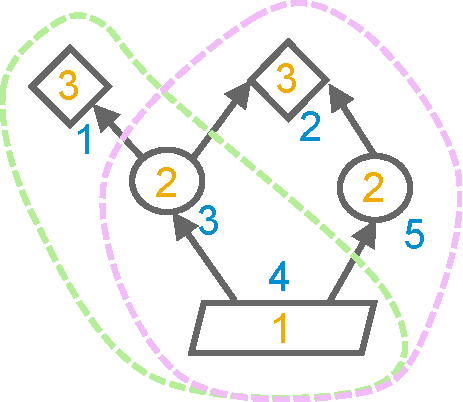
\includegraphics[width=0.30\textwidth]{Bilder/problem_illustration.pdf}
% 	\vspace{-10pt}
% 	% Das folgende ist ein Trick, um "Abbilgung x.y" in eine
% 	% eigene Zeile zu packen. Der Text zwischen [ und ] steht
% 	% im Abbildungsverzeichnis. Der Text darunter wird
% 	% tatsächlich angezeigt.
% 	\caption[Minimalbeispiel zur Teilgraph-Überspringungs-Problematik. Legende wie in \autoref{fig:trans_closures}.]{\unskip}
% 	Minimalbeispiel zur Teilgraph-Überspringungsproblematik. Legende wie in Abb. \ref{fig:trans_closures}.
% 	\label{fig:prob_illu}
% \end{wrapfigure}

% Leider lassen sich bei dem Vergleich zweier Submodelle gemeinsame Teilgraphen nicht gänzlich einsparen, indem der Similarity-Wert über Forks hinaus propagiert wird, um so jedem Knoten im Graph die Summe aller Knotenwerte unter ihm zuzuordnen, da ein gemeinsamer Teilgraph über mehrere Forks betreten werden kann (z.B. der Teilgraph der Schnittmenge von grün und lila in \autoref{fig:trans_closures} kann über Knoten 6 und 5 betreten werden) und nur der maximale Teilgraph gezählt werden darf - ansonsten würde es zu einer doppelten Wertung eines oder mehrerer Knoten kommen. Auch ist die Maximalität  des gemeinsamen Teilgraphen nur mit erheblichen Rechenaufwand, der dem Prinzip des Auslassens entgegensteht, zu überprüfen. Der Graph aus \autoref{fig:prob_illu} ist zur Veranschaulichung geeignet: Es ist schwierig Knoten 4 mit Wert 1 genau einmal zu zählen. Wird Knoten 3 betreten und der restliche Teilgraph (Knoten 4) übersprungen, so wird der Wert 3 zur Similarity addiert.
